\section{Branches}\label{sec:branch}
Während der Entwicklung eines Programms ist es meist nützlich mehrere Versionen parallel zu verwalten. Das kann heißen, dass es eine \qq{release} Version und eine \qq{developement} Version gibt oder, dass man die letzte funktionierende Variante des Programms erhalten will während man neue Funktionen versucht zu implementieren.

Die parallele Entwicklung an mehreren Versionen wird durch Branches ermöglicht.
\subsection{Branch erstellen}
Um einen Branch zu erstellen wird \inline{git branch [Name]}, mit einem Namen für den Branch, genutzt. Mit \inline{git checkout} wird der aktive Branch ausgewählt. Der Log zeigt den Verlauf, des gerade aktiven Branches an.
\begin{mplisting}
$ git branch section4
$ git checkout section4
$ git log --pretty=format:"%h %s %d"
04965ab add: sentence at end of Commit  (HEAD -> section4, master)
906a721 add: label for future sections 
03a1fee add: Subsection about reverting commits 
bf11cfe add: files to ignore from macOS 
\end{mplisting}
Hier kann man sehen, dass sowohl \inline{master}, als auch \inline{section4} auf denselben Commit zeigen (\inline{04965ab}). Jeder neue Commit jedoch wird nur von dem Branch erfasst, auf den \inline{HEAD} zeigt (\inline{section4}).

\begin{figure}[!h]
	\centering
	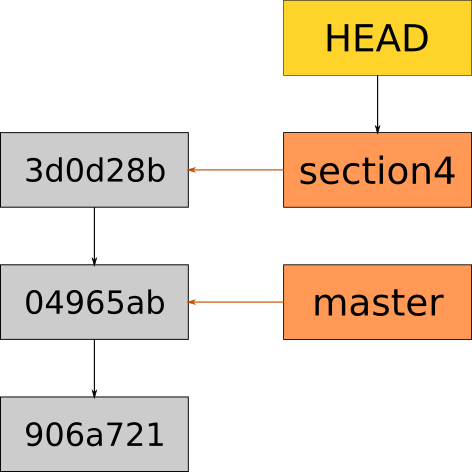
\includegraphics[width=0.4\textwidth]{Bilder/branching.png}
	\caption{Beispielhafter Commit-Baum aus diesem Projekt. Graue Kästen stellen einzelne Commits dar, orangene Branches und der gelbe Kasten ist der aktuelle HEAD. Die Pfeile zeigen auf die Verlinkung.}
	\label{fig:branch_1}
\end{figure}
Abb. \ref{fig:branch_1} zeigt den Commit-Baum des Repositories nach dem ersten Commit in \inline{section4}. \inline{HEAD} zeigt auf den aktuellen Zustand des lokalen Ordners. In diesem Fall auf den Branch \inline{section4}. Die Branches selber zeigen auf den Commit, den sie gerade darstellen. Um den \inline{HEAD} zu wechseln muss nur \inline{git checkout [BRANCH]} mit dem entsprechenden Branch aufgerufen werden.
\begin{figure}[!h]
	\centering
	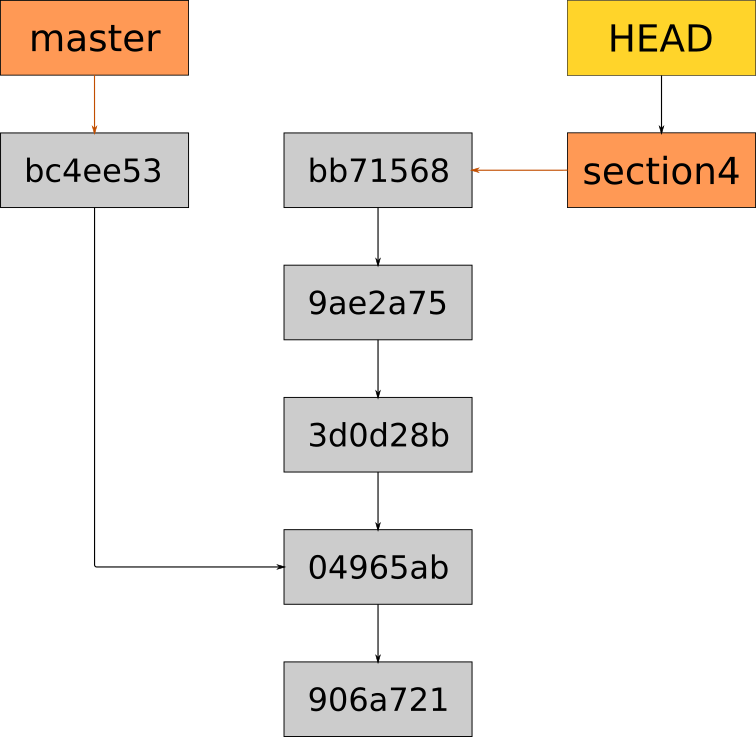
\includegraphics[width=0.4\textwidth]{Bilder/branching_2.png}
	\caption{Branch-tree nachdem mehrere Commits zu den Branches gemacht wurden.}
	\label{fig:branch_2}
\end{figure}

\subsection{Merging}
Das Zusammenführen zweier Branches wird Merging genannt. Dabei ist das Ziel, alle Änderungen der beiden Branches zu vereinen. Wichtig ist, dass immer der Branch ausgewählt (\inline{HEAD} zeigt darauf) sein sollte, in dem die Änderungen vereint werden sollen. Will man also in \inline{master} die Änderungen von \inline{section4} einbinden geht das folgendermaßen:
\begin{mplisting}
$ git checkout master
$ git merge section4
Merge made by the 'recursive' strategy.
Bilder/branching.png   | Bin 0 -> 25763 bytes
Bilder/branching.svg   | 648 +++++++++++++++++++++++++++++++++++
Bilder/branching_2.png | Bin 0 -> 41671 bytes
branches.tex           |  36 +++++
main.tex               |   3 +-
5 files changed, 686 insertions(+), 1 deletion(-)
create mode 100644 Bilder/branching.png
create mode 100644 Bilder/branching.svg
create mode 100644 Bilder/branching_2.png
create mode 100644 branches.tex
\end{mplisting}
Durch das mergen wird ein neuer Commit angelegt, welcher auf beide  \qq{parents} verweist (vgl. Abschnitt \ref{sec:first_commit}, statt einem \qq{parent} hat dieser Commit zwei). Nachdem ein Branch gemerged wurde kann er gelöscht werden.
\begin{figure}[!ht]
	\centering
	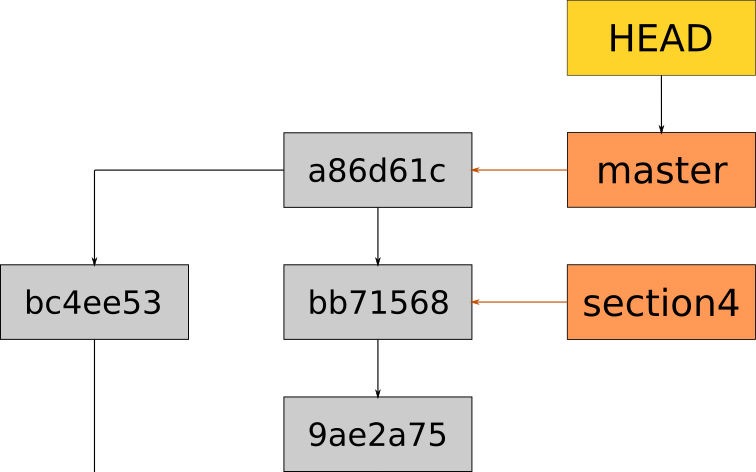
\includegraphics[width=0.6\textwidth]{Bilder/branching_3.png}
	\caption{Commit-Baum nach dem Merging. Der Merge wird als eigener Commit oberhalb der beiden \qq{parent}-Commits angezeigt. Der \inline{master} Branch und \inline{HEAD} zeigen beide auf den Merge-Commit. Der \inline{section4} Branch existiert weiterhin, zeigt jedoch auf den alten Commit.}
	\label{fig:merge}
\end{figure}

% MERGE Conflicts missing